% Created 2018-10-16 ti. 14:00
\documentclass{article}
\usepackage[utf8]{inputenc}
\usepackage[T1]{fontenc}
\usepackage{fixltx2e}
\usepackage{graphicx}
\usepackage{longtable}
\usepackage{float}
\usepackage{wrapfig}
\usepackage{rotating}
\usepackage[normalem]{ulem}
\usepackage{amsmath}
\usepackage{textcomp}
\usepackage{marvosym}
\usepackage{wasysym}
\usepackage{amssymb}
\usepackage{hyperref}
\tolerance=1000
\usepackage{tikz,wrapfig} \usetikzlibrary{calligraphy,calc,patterns,angles,quotes,decorations.pathreplacing,intersections} \usetikzlibrary{decorations.pathreplacing,calligraphy}
\date{}
\title{1T}
\hypersetup{
  pdfkeywords={},
  pdfsubject={},
  pdfcreator={Emacs 24.5.1 (Org mode 8.2.10)}}
\begin{document}

\maketitle

\section{Arealsetningen}
\label{sec-1}
Idag skal vi lære om arealsetningen

Gitt en trekant $ABC$ der vi kjenner lengdene $q=AB$, $p=AC$ der vinkelen mellom disse er $\theta$, da har vi at arealet $A$ er gitt ved:
\[
A = \frac{1}{2}pq\sin{\theta}
\]
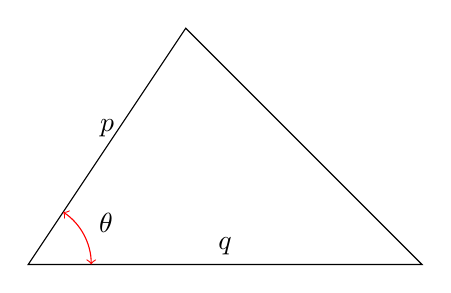
\begin{tikzpicture}
  \draw
    (0,0) coordinate (A) 
    -- (2,3) coordinate (B) node[midway,above,align = center] {$p$}
    -- (5,0) coordinate (C)
    -- cycle  node[midway, above] {$q$}
    pic["$\theta$", draw=red, <->, angle eccentricity=1.4, angle radius=0.8cm]
    {angle=C--A--B};
\end{tikzpicture}


\subsection{Eksempel 1:}
\label{sec-1-1}
\begin{figure}[h!]
\centering
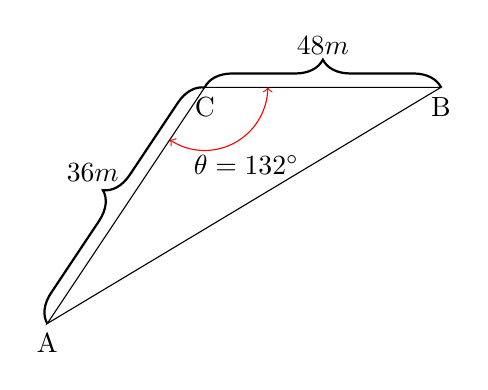
\begin{tikzpicture}
  \draw
    (0,0) coordinate (A) node[below] {A}
    -- (2,3) coordinate (C) node[below] {C}
    -- (5,3) coordinate (B) node[below] {B}
    -- cycle
    pic["$\theta = 132^{\circ}$", draw=red, <->, angle eccentricity=1.4, angle radius=0.8cm]
    {angle=A--C--B};
    \draw[decorate,decoration={brace,amplitude=10pt},yshift=0pt,thick] (A) -- (C) node [midway,yshift=12pt, xshift =-12pt]{$36m$};
    \draw[decorate,decoration={brace,amplitude=10pt},yshift=0pt,thick] (C) -- (B) node [midway,yshift=15pt, xshift =0pt]{$48m$};
\end{tikzpicture}
\end{figure}
Vi vil regne ut arealet av tomta som er gitt i figuren ved siden av.
Vi kjenner vinkelen mellom de to sidene samt lengen. Da bruker vi sinussetningen til å vise at :
\[
A = \frac{1}{2} AC \cdot BC \cdot \sin{\theta} = \frac{1}{2} 36 \cdot 48 \cdot \sin{132} \approx 640.
\]
\subsection{Bevis}
\label{sec-1-2}
Del beviset inn i 2 deler
\subsubsection{$\theta < 90^{\circ}$}
\label{sec-1-2-1}
\begin{itemize}
\item Trekk en linje $h$ ned langs midten.
\item Utrykk $h$ ved hjelp av $\sin{\theta}$ og $q$.
\item Plugg inn i formel for areal.
\end{itemize}
\subsubsection{$\theta > 90^{\circ}$}
\label{sec-1-2-2}
\begin{itemize}
\item Trekk en linje ned fra toppen og dann en rettviklet trekant.
\item Finn $h$ ved hjelp av supplementvinkelen til $\theta$.
\item plugg dette inn i formelen for areal.
\end{itemize}
\subsection{Eksemepel 2}
\label{sec-1-3}
Finn alle trekanter $ABC$ med areal lik $3.5cm$ der $AB = 3.2cm$ og $AC = 2.5cm$. 
Vi bruker formelen og finner at $\theta = 61^{\circ}$ og finner supplementvinkelen.

\section{Cosinus setningen}
\label{sec-2}
Gitt en trekant som ikke er nødvendigivis rettvinklet. Da har vi at:
\[
a^2 = b^2 + c^2 -2bc \cos{\theta}
\]

\subsection{Eksempel 1}
\label{sec-2-1}
\begin{figure}[h!]
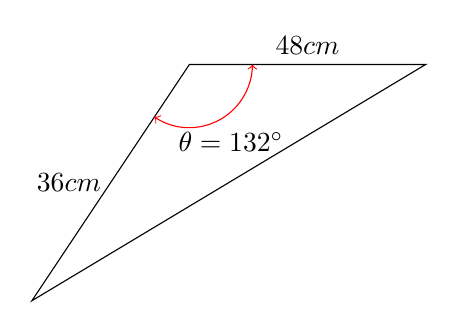
\begin{tikzpicture}
  \draw
    (0,0) coordinate (A) 
    -- (2,3) coordinate (B) node[midway,left,align = center] {$36cm$}
    -- (5,3) coordinate (C) node [midway, above] {$48cm$}
    -- cycle
    pic["$\theta=132^{\circ}$", draw=red, <->, angle eccentricity=1.4, angle radius=0.8cm]
    {angle=A--B--C};
\end{tikzpicture}
\end{figure}
I denne figuren kjenner vi to sider og vinkelen mellom sidene. 
Vi kan da bruke cosinussetningen til å finne ut av hva den siste siden må være. 
\begin{align*}
x^2 & = 36^2 + 48^2 -2\cdot 36 \cdot 48 \cdot \cos{132^{\circ}} \approx 5912,5\\
x & = \sqrt{5912,5} \approx 77
\end{align*}

\subsection{Bevis}
\label{sec-2-2}
Dette er kun bevist for $\theta <90^{circ}$ For trekanten $ABC$ der $\theta$ tilhører \$A\$\\
\begin{itemize}
\item Trekk først en linje ned fra $C$ ned til $A$ og la $x$ være avastenden fra der denne linja treffer $AB$.
\item Observer så at
\end{itemize}
\[
b^2 = x^2 + h^2 \hspace{5mm} \cos{\theta} = \frac{x}{b} \hspace{5mm} x = b\cos{\theta}
\]
Bruk pythagorias til å vise at $a^2 = h^2 + (c-x)^2$. 
Da får vi at $a^2 = h^2 +c^2 -2cx + x^2 = b^2 +c^2 -2cb\cos{\theta}$ \newline
For å komme frem til dette er stattet vi $h^2 +x^2$ med $b^2$ og brukte at $x=b\cos{\theta}$
% Emacs 24.5.1 (Org mode 8.2.10)
\end{document}